%% Source of figures/empirical-measures.pdf. Compile: pdflatex empirical-measures.tex
%% Generated 2026-10-28 from the SMOTE25 evaluation draft page (76 coded papers, 71 empirical).
%% Numbers are filled from the coded data; regenerate instead of editing them by hand.
\documentclass[border=4pt]{standalone}
\usepackage[scaled]{helvet}\renewcommand{\familydefault}{\sfdefault}
\usepackage{pgfplots}\pgfplotsset{compat=1.18}
\definecolor{sOne}{HTML}{2A78D6}\definecolor{sTwo}{HTML}{EB6834}\definecolor{sThree}{HTML}{1BAF7A}\definecolor{sFour}{HTML}{EDA100}
\definecolor{oZero}{HTML}{A3ABB4}\definecolor{oOne}{HTML}{5598E7}\definecolor{oTwo}{HTML}{1C5CAB}\definecolor{oThree}{HTML}{0D366B}\definecolor{inkTwo}{HTML}{465462}
\begin{document}
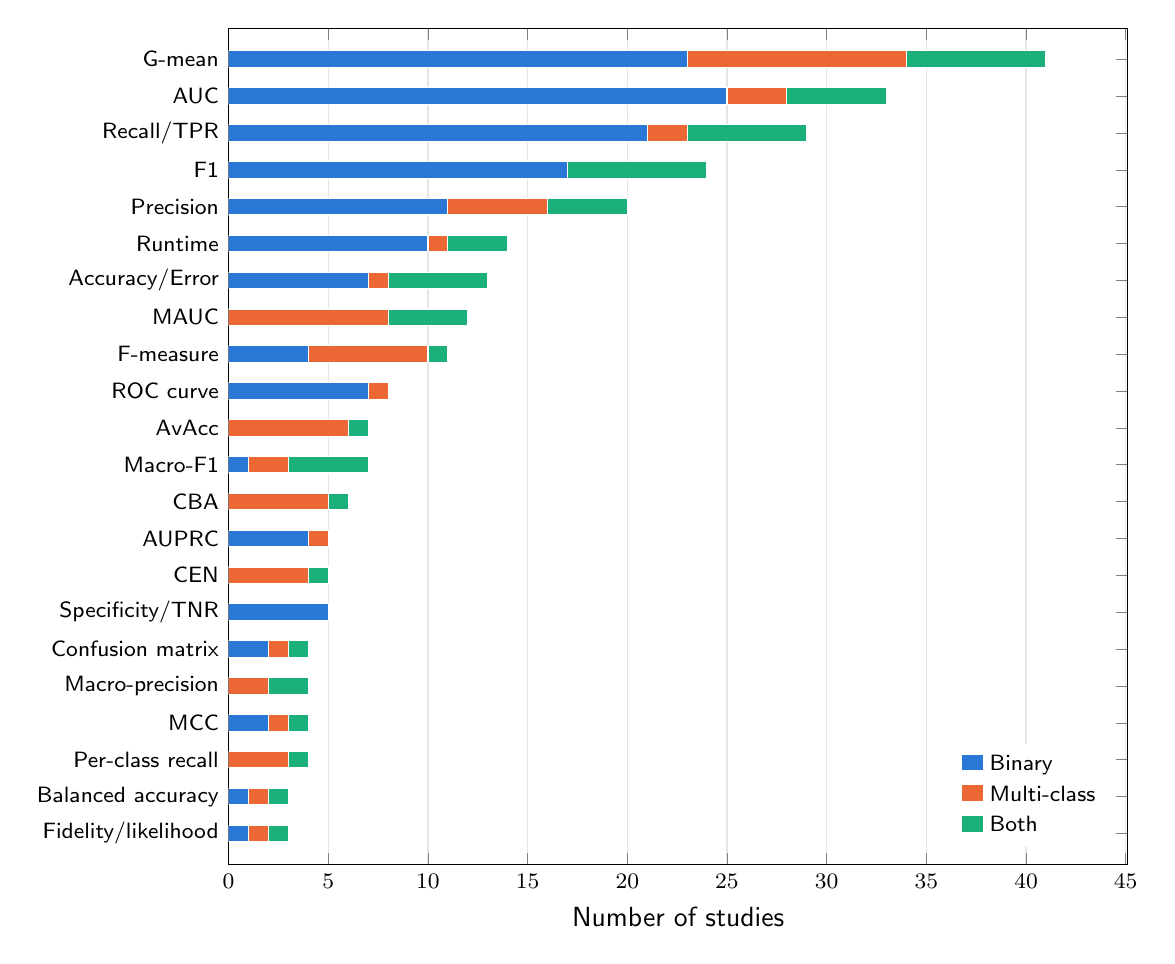
\begin{tikzpicture}
\begin{axis}[xbar stacked,width=13cm,height=12.2cm,bar width=6pt,xmin=0,y dir=reverse,ytick={0,...,21},
  yticklabels={{G-mean},{AUC},{Recall/TPR},{F1},{Precision},{Runtime},{Accuracy/Error},{MAUC},{F-measure},{ROC curve},{AvAcc},{Macro-F1},{CBA},{AUPRC},{CEN},{Specificity/TNR},{Confusion matrix},{Macro-precision},{MCC},{Per-class recall},{Balanced accuracy},{Fidelity/likelihood}},xlabel={Number of studies},enlarge y limits=0.04,
  tick label style={font=\footnotesize},legend cell align=left,legend style={font=\footnotesize,at={(0.98,0.02)},anchor=south east,draw=none},xmajorgrids,grid style={gray!20}]
\addplot[fill=sOne,draw=white] coordinates {(23,0) (25,1) (21,2) (17,3) (11,4) (10,5) (7,6) (0,7) (4,8) (7,9) (0,10) (1,11) (0,12) (4,13) (0,14) (5,15) (2,16) (0,17) (2,18) (0,19) (1,20) (1,21)};
\addplot[fill=sTwo,draw=white] coordinates {(11,0) (3,1) (2,2) (0,3) (5,4) (1,5) (1,6) (8,7) (6,8) (1,9) (6,10) (2,11) (5,12) (1,13) (4,14) (0,15) (1,16) (2,17) (1,18) (3,19) (1,20) (1,21)};
\addplot[fill=sThree,draw=white] coordinates {(7,0) (5,1) (6,2) (7,3) (4,4) (3,5) (5,6) (4,7) (1,8) (0,9) (1,10) (4,11) (1,12) (0,13) (1,14) (0,15) (1,16) (2,17) (1,18) (1,19) (1,20) (1,21)};
\legend{{Binary},{Multi-class},{Both}}
\end{axis}
\end{tikzpicture}
\end{document}
